\documentclass[tikz,border=6pt]{standalone}
\usepackage{amsmath,xcolor}
\usetikzlibrary{arrows.meta,positioning,fit}
\definecolor{navy}{HTML}{254B6E}
\definecolor{blue}{HTML}{4D83AE}
\definecolor{teal}{HTML}{2A8791}
\definecolor{green}{HTML}{3B806E}
\definecolor{ink}{HTML}{263746}
\definecolor{muted}{HTML}{5D6C78}
\definecolor{paleBlue}{HTML}{EAF2F7}
\definecolor{paleTeal}{HTML}{E8F3F2}
\definecolor{paleGray}{HTML}{F4F6F7}
\definecolor{border}{HTML}{C7D2D9}
\tikzset{
  >={Stealth[length=2.2mm]},
  panel/.style={font=\sffamily\bfseries\large,text=ink},
  paneltag/.style={circle,fill=navy,text=white,font=\sffamily\bfseries,inner sep=2pt,minimum size=6mm},
  stage/.style={rounded corners=2mm,draw=border,fill=paleGray,minimum width=2.35cm,minimum height=1.45cm,align=center,text=ink,font=\sffamily},
  target/.style={rounded corners=2mm,draw=blue,fill=paleBlue,minimum width=2.35cm,minimum height=1.45cm,align=center,text=navy,font=\sffamily},
  finetune/.style={rounded corners=2mm,draw=teal,fill=paleTeal,minimum width=2.35cm,minimum height=1.45cm,align=center,text=ink,font=\sffamily},
  tiny/.style={font=\sffamily\small,text=muted,align=center},
  arrow/.style={-{Stealth[length=2.2mm]},draw=teal,line width=1.1pt}
}
\begin{document}
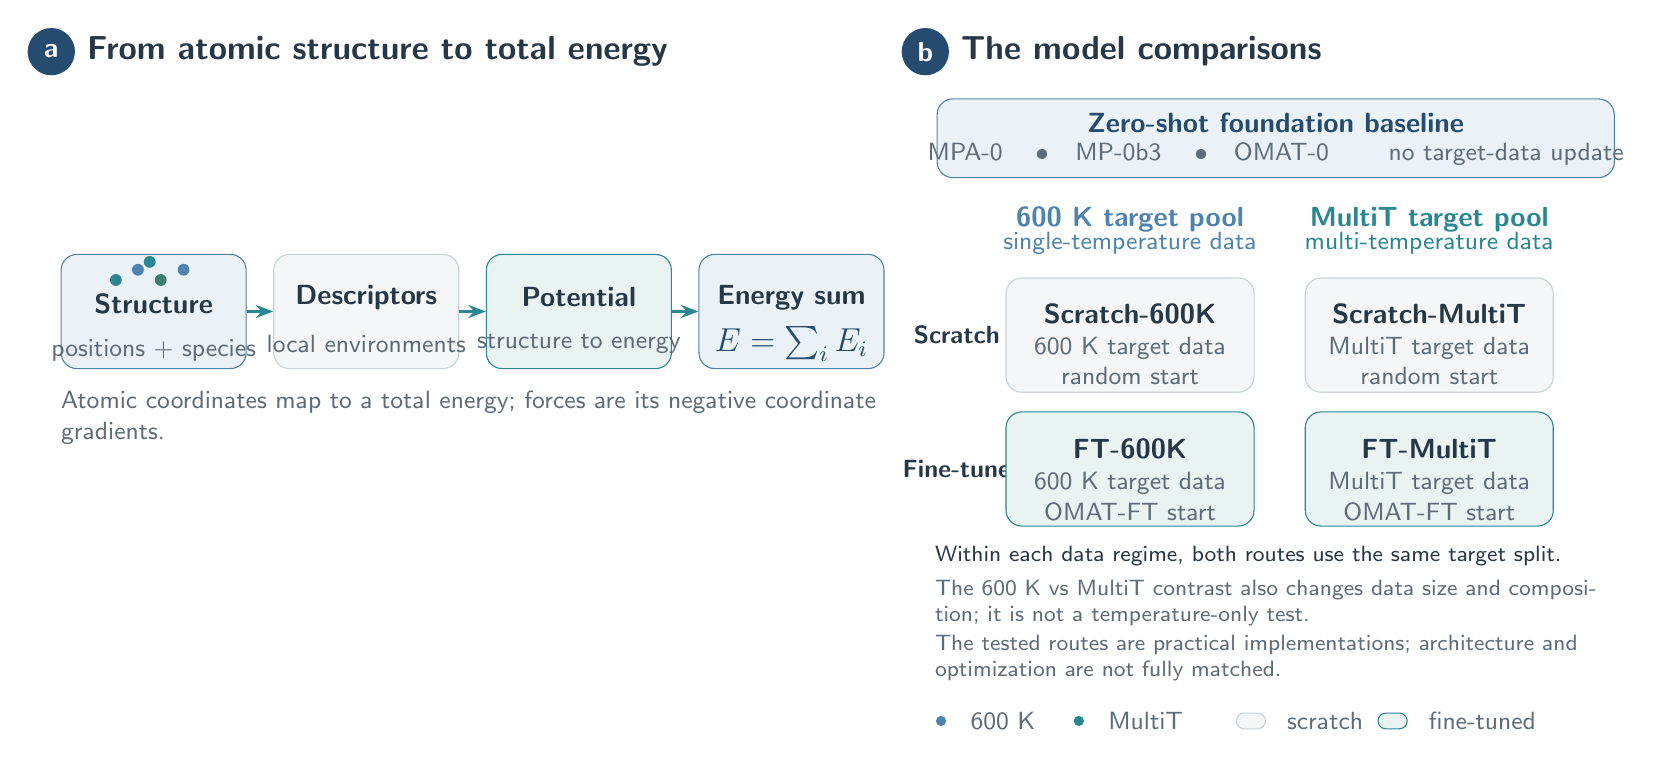
\begin{tikzpicture}[x=1cm,y=1cm]
% Panel A: energy model
\node[paneltag] at (0.45,9.55) {a};
\node[panel,anchor=west] at (0.78,9.55) {From atomic structure to total energy};

\node[target] (structure) at (1.75,6.25) {};
\node[font=\sffamily\bfseries,text=ink] at (1.75,6.35) {Structure};
\node[tiny] at (1.75,5.75) {positions + species};
\foreach \x/\y/\c in {1.27/6.65/teal,1.55/6.78/blue,1.84/6.65/green,2.13/6.78/blue,1.7/6.88/teal}
  \fill[\c] (\x,\y) circle (0.075);

\node[stage] (descriptor) at (4.45,6.25) {};
\node[font=\sffamily\bfseries,text=ink] at (4.45,6.43) {Descriptors};
\node[tiny] at (4.45,5.84) {local environments};

\node[finetune] (model) at (7.15,6.25) {};
\node[font=\sffamily\bfseries,text=ink] at (7.15,6.43) {Potential};
\node[tiny] at (7.15,5.84) {structure to energy};

\node[target] (energy) at (9.85,6.25) {};
\node[font=\sffamily\bfseries,text=ink] at (9.85,6.43) {Energy sum};
\node[font=\sffamily\large,text=navy] at (9.85,5.84) {$E=\sum_i E_i$};

\draw[arrow] (structure.east) -- (descriptor.west);
\draw[arrow] (descriptor.east) -- (model.west);
\draw[arrow] (model.east) -- (energy.west);

\node[tiny,anchor=west,text width=10.7cm,align=left] at (0.45,4.9)
{Atomic coordinates map to a total energy; forces are its negative coordinate gradients.};

% Panel B: comparison structure
\node[paneltag] at (11.55,9.55) {b};
\node[panel,anchor=west] at (11.88,9.55) {The model comparisons};

\node[rounded corners=2mm,draw=blue,fill=paleBlue,minimum width=8.6cm,minimum height=1.0cm,align=center] (zero) at (16.0,8.45) {};
\node[font=\sffamily\bfseries,text=navy] at (16.0,8.65) {Zero-shot foundation baseline};
\node[font=\sffamily\small,text=muted] at (16.0,8.25) {MPA-0 \quad\textbullet\quad MP-0b3 \quad\textbullet\quad OMAT-0 \qquad no target-data update};

\node[font=\sffamily\bfseries,text=blue,align=center] at (14.15,7.42) {600 K target pool};
\node[font=\sffamily\bfseries,text=teal,align=center] at (17.95,7.42) {MultiT target pool};
\node[font=\sffamily\small,text=blue,align=center] at (14.15,7.12) {single-temperature data};
\node[font=\sffamily\small,text=teal,align=center] at (17.95,7.12) {multi-temperature data};

\node[font=\sffamily\bfseries\small,text=ink,align=center] at (11.95,5.95) {Scratch};
\node[font=\sffamily\bfseries\small,text=ink,align=center] at (11.95,4.25) {Fine-tune};

\node[stage,minimum width=3.15cm,minimum height=1.45cm] at (14.15,5.95) {};
\node[font=\sffamily\bfseries,text=ink] at (14.15,6.22) {Scratch-600K};
\node[tiny] at (14.15,5.62) {600 K target data\\random start};

\node[stage,minimum width=3.15cm,minimum height=1.45cm] at (17.95,5.95) {};
\node[font=\sffamily\bfseries,text=ink] at (17.95,6.22) {Scratch-MultiT};
\node[tiny] at (17.95,5.62) {MultiT target data\\random start};

\node[finetune,minimum width=3.15cm,minimum height=1.45cm] at (14.15,4.25) {};
\node[font=\sffamily\bfseries,text=ink] at (14.15,4.50) {FT-600K};
\node[tiny] at (14.15,3.90) {600 K target data\\OMAT-FT start};

\node[finetune,minimum width=3.15cm,minimum height=1.45cm] at (17.95,4.25) {};
\node[font=\sffamily\bfseries,text=ink] at (17.95,4.50) {FT-MultiT};
\node[tiny] at (17.95,3.90) {MultiT target data\\OMAT-FT start};

\node[tiny,anchor=west,text width=8.6cm,align=left,font=\sffamily\footnotesize,text=ink] at (11.55,3.15)
{Within each data regime, both routes use the same target split.};
\node[tiny,anchor=west,text width=8.6cm,align=left,font=\sffamily\footnotesize] at (11.55,2.55)
{The 600 K vs MultiT contrast also changes data size and composition; it is not a temperature-only test.};
\node[tiny,anchor=west,text width=8.6cm,align=left,font=\sffamily\footnotesize] at (11.55,1.85)
{The tested routes are practical implementations; architecture and optimization are not fully matched.};

\fill[blue] (11.75,1.05) circle (0.065);
\node[tiny,anchor=west] at (12.00,1.05) {600 K};
\fill[teal] (13.50,1.05) circle (0.065);
\node[tiny,anchor=west] at (13.75,1.05) {MultiT};
\draw[rounded corners=1mm,draw=border,fill=paleGray] (15.50,0.95) rectangle (15.87,1.15);
\node[tiny,anchor=west] at (16.02,1.05) {scratch};
\draw[rounded corners=1mm,draw=teal,fill=paleTeal] (17.30,0.95) rectangle (17.67,1.15);
\node[tiny,anchor=west] at (17.82,1.05) {fine-tuned};
\end{tikzpicture}
\end{document}
